\documentclass{article}

% if you need to pass options to natbib, use, e.g.:
%     \PassOptionsToPackage{numbers, compress}{natbib}
% before loading neurips_2020

% ready for submission
% \usepackage{neurips_2020}

% to compile a preprint version, e.g., for submission to arXiv, add add the
% [preprint] option:
%     \usepackage[preprint]{neurips_2020}

% to compile a camera-ready version, add the [final] option, e.g.:
%     \usepackage[final]{neurips_2020}

% to avoid loading the natbib package, add option nonatbib:
     \usepackage[preprint]{neurips_2020}

\usepackage[utf8]{inputenc} % allow utf-8 input
\usepackage[T1]{fontenc}    % use 8-bit T1 fonts
\usepackage{hyperref}       % hyperlinks
\usepackage{url}            % simple URL typesetting
\usepackage{booktabs}       % professional-quality tables
\usepackage{amsfonts}       % blackboard math symbols
\usepackage{nicefrac}       % compact symbols for 1/2, etc.
\usepackage{microtype}      % microtypography
\usepackage{listings}
\usepackage{graphicx}
\usepackage{subfigure}

\title{Programming Assignment \#1 of WI 21 CSE 251B}

% The \author macro works with any number of authors. There are two commands
% used to separate the names and addresses of multiple authors: \And and \AND.
%
% Using \And between authors leaves it to LaTeX to determine where to break the
% lines. Using \AND forces a line break at that point. So, if LaTeX puts 3 of 4
% authors names on the first line, and the last on the second line, try using
% \AND instead of \And before the third author name.

\author{%
  Fangzhou Ai\\
  Department of Electrical and Computer Engineering\\
  University of California, San Diego\\
  La Jolla, CA 92093 \\
  \texttt{faai@eng.ucsd.edu} \\
  % examples of more authors
   \And
   Yue Qiao \\
   Department of Electrical and Computer Engineering \\
   University of California, San Diego\\
   La Jolla, CA 92093 \\
   \texttt{yuq021@eng.ucsd.edu}
}

\begin{document}

\maketitle

\begin{abstract}
  This paper is a report for the programming assignment 1 for Lecture CSE 251B.
\end{abstract}

\section{Load and preprocess the data}
\label{Sec:LPD}
\paragraph{Load data} Data loading cold be done by easily calling the given function load\_data();

\paragraph{Preprocess data} After loading the data, we get a dictionary contains 4 different kinds of cars, the keys are the cars' names and values are a list contains a series of images, we also get a dictionary cnt which include how many images we have within each car's category. To turn the data into a more convenient form for training, we did the following things: 1. turn the list into a Numpy array for more fancy matrix operations and 2. we write our own label encoding program to turn each category into a vector (eg. 'Minivan' would be [0, 1, 0, 0]).

\section{Cross validation procedure}
\label{Sec:CVP}
\paragraph{Split the data} Notice that ideally we want to split the data in a way that each type of car would evenly distributed within training set, validations set and test set, by looking at our database, we found that each category has almost the same number of pictures(Convertible: 149 \# of images, Minivan: 148 \# of images, Pickup: 150 \# of images, Sedan: 150 \# of images), therefore we choose to split each set into k parts then combine them together to form the new data set, in which case we can guarantee that each part would evenly contains all types of cars.

\paragraph{Cross validation} To make sure each part would be test set once and validation set once, we maintained an index array [0, 1,...., k - 1], the first element indicate the index of test set, the second element indicate the index of validations set, the rest elements indicate the training set, after each training procedure, we let each element pump 1 then mod k, so the first time the test set would be the part 0, validation set is part 1, training set is 2 to k -1, the second time the test set would be the part 1, validation set is part 2, training set is [3, 4,..., k - 1, 0], at the last training procedure the test set would be the part k - 1, validation set is part 0, training set is 1 to k - 2. Hence each set has been set to test set and validations set once.

\section{Principal components analysis}
\label{Sec:PCA}

\paragraph{Implement PCA} The verified mean and std on each set is shown in \autoref{tab:pca}.

\begin{table}
	\caption{Mean and std of different set.}
	\label{tab:pca}
	\centering
	\begin{tabular}{lll}
		\toprule
		Set     & Mean     & STD \\
		\midrule
		Training & 4.65502e-20  & 0.999999     \\
		Validation     & -0.00031 & 0.860112      \\
		test     & -0.00054      & 0.833020  \\
		\bottomrule
	\end{tabular}
\end{table}


\section{Logistic regression}
Logistic model is a very simple model which has only one output and use sigmoid as the activation function. It can only identify 2 different objects while it's simplicity make it a very popular toy model to understand the principle behind machine learning. Here we use python with only Numpy library to build a trivial program to implement this model's key idea.
\label{Sec:LR}
\subsection{(a)} The logistic regression code is shown in \autoref{lst:LR}. We only need one output because we only have 2 categories, if we assume the output is the probability of the first category, then the probability for the second one is naturally 1 - p.
\lstset{language=Python}
\lstset{frame=lines}
\lstset{caption={Logistic regression implementation}}
\lstset{label={lst:LR}}
\lstset{basicstyle=\footnotesize}
\begin{lstlisting}
	import numpy as np
	def simple_logistic_model(w, input):
	''' logistic model withou hidden layer
	Args:
		input, which dimention is M * (1 + d), means M pics 
		each pixel number is d, appnded by 1
		w, parameters, dimention of d + 1 * 1
	Returns:
		x, dimention of M * 1
	'''
		x = np.dot(input, w)
		x = 1/(1 + np.exp(-x)) 
		return x
\end{lstlisting}
\subsection{(b)}
The loss of the validation set is shown in Fig 1. And the accuracy on test set is around 63.33\%, the validation loss clearly shows the overfiting problem here that loss goes down quickly at first then goes up. Here we have 40 PCA components. Looking at the PCA components(the first 4 are shown in Fig 2), we found that since the objects are not aligned, it's very hard for PCA to get accurate car's shape, thus not able to achieve high accuracy. 
\begin{figure}
	\centering
	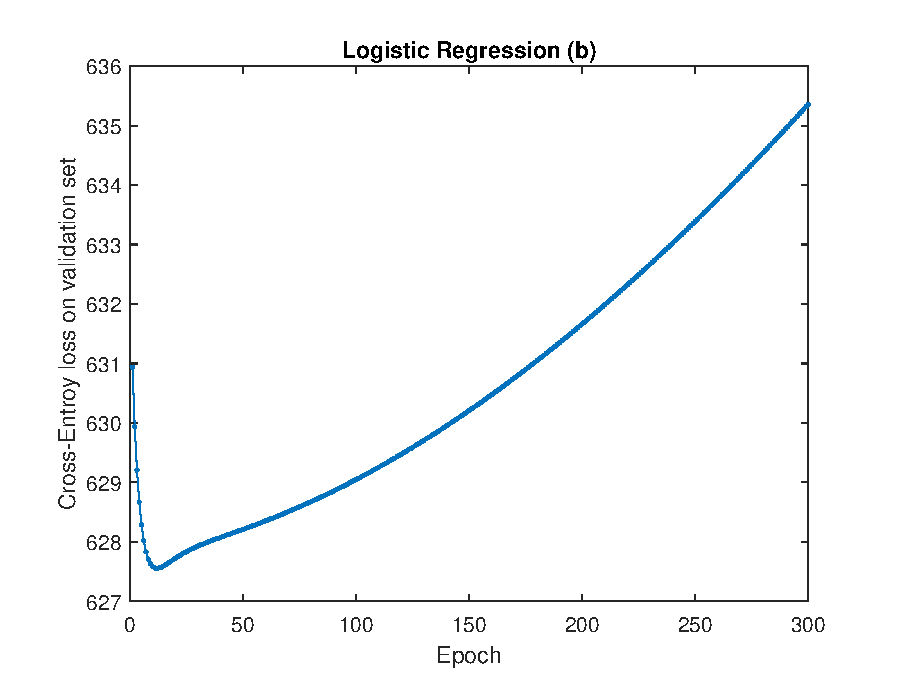
\includegraphics[width = 8cm]{LR(b)00.eps}
	\label{fig:1}
	\caption{Cross entropy loss on validation set}
\end{figure}

\begin{figure*}
	
	\centering
	\subfigure{
	\begin{minipage}[b]{0.45\linewidth}
			\includegraphics[width=1\linewidth]{LR(b)01.png}\vspace{4pt}
			\includegraphics[width=1\linewidth]{LR(b)02.png}
	\end{minipage}}
	\subfigure{
	\begin{minipage}[b]{0.45\linewidth}
			\includegraphics[width=1\linewidth]{LR(b)03.png}\vspace{4pt}
			\includegraphics[width=1\linewidth]{LR(b)04.png}
	\end{minipage}}
	\label{fig:2}
	\caption{First 4 PCA components.}
\end{figure*}

\subsection{(c)}
By alternating the data source from resized to aligned, we see a a huge improvement on accuracy, the accuracy we achieved here is 83.5\% with 300 epochs. The mean and std of accuracy and loss is shown in Figure 3. We also try different laearning rate here, one is too large, one is too small and a normal one, the difference is shown in Figure 4. As we can see that a large learning rate may lead to strong oscillation while a small one would lead to a slow converging speed.

\begin{figure}
	
	\centering
	\subfigure{
			\includegraphics[width=0.5\linewidth]{LR(c)01.png}
			\includegraphics[width=0.5\linewidth]{LR(c)02.png}
		}
	\label{fig:3}
	\caption{Mean and std of accuracy and loss, classification between Convertible and Minivan.}
\end{figure}

\begin{figure}
	\centering
	\includegraphics[width = 0.8\linewidth]{LR(c)DiffLR.png}
	\caption{Different learning rate effects on training loss.}
\end{figure}


\subsection{(d)}
The classification accuracy between category Pickup and Sedan is 82.67\%, namely, we didn't notice any significant differences between different category classification tasks, Which is reasonable since this logistic model is simple yet powerful enough to generalized to similar objects. The mean and std of training loss is shown in Figure 5.

\begin{figure}
	
	\centering
	\subfigure{
		\includegraphics[width=0.5\linewidth]{LR(c)03.png}
		\includegraphics[width=0.5\linewidth]{LR(c)04.png}
	}
	\label{fig:3}
	\caption{Mean and std of accuracy and loss, classification between Pickup and Sedan.}
\end{figure}





\section{Softmax regression}
\label{Sec:SR}



\section{Individual contributions to the project}
\label{Sec:ICP}
Fangzhou Ai: Logistic regression.
Yue Qiao: Softmax regression, code refactor.

\end{document}